\section{Liniendiagrammsklassifizierung}
\label{ch:classify_eval}

Für die Liniendiagrammsklassifizierung wurden zwei Modelle jeweils auf die erstellten Datensätze aus \ref{ch:linebank} trainiert. Die Konfusionsmatrix \ref{fig:val_v1_matrix} macht die Schwierigkeit des Modells deutlich, überlappende und nicht überlappende Liniendiagramme zu differenzieren. Im Gegensatz zu \ref{fig:val_v2_matrix} werden hier 7 der insgesamt 19 nicht überlappenden Aufkommen falsch als überlappende Diagramme klassifiziert.

\begin{figure}[H]
    \centering
    \captionsetup{width=.75\linewidth}
    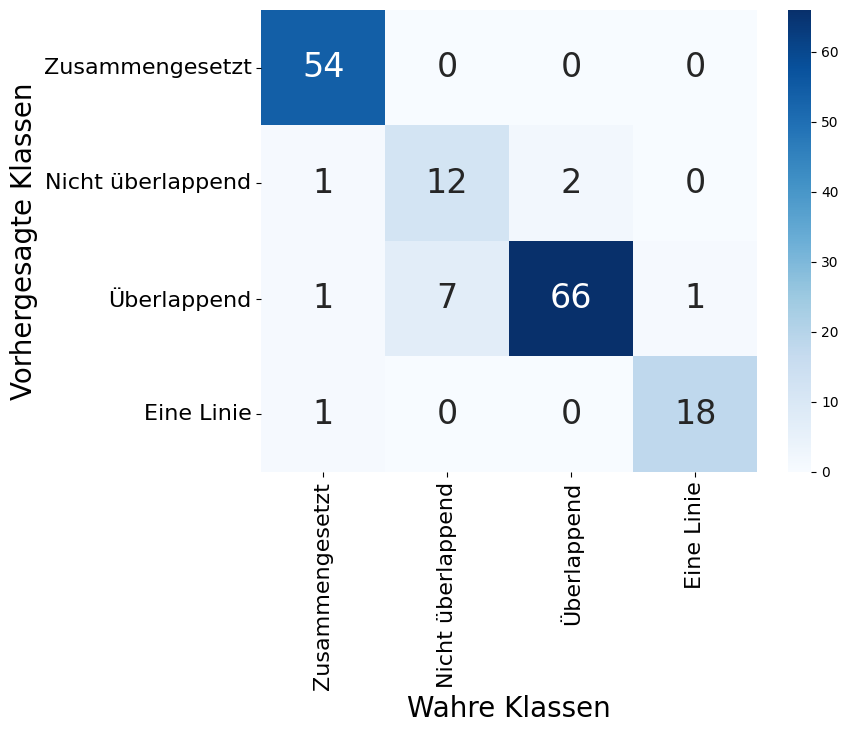
\includegraphics[width=.75\textwidth]{Experimente/img/classify/val_v1/matrix.png}
    \caption{\hbadness=10000 x}
    \label{fig:val_v1_matrix}
\end{figure}

Die besseren Ergebnisse der Unterscheidung zwischen einer und mehreren Wertelinien dagegen, spiegelt sich aber auch in der Accuracy wider: Statt 92.0\% des ersten Modells erziehlte dieses eine Klassifikationsgenauigkeit von 98.1\%.

\begin{figure}[H]
    \centering
    \captionsetup{width=.75\linewidth}
    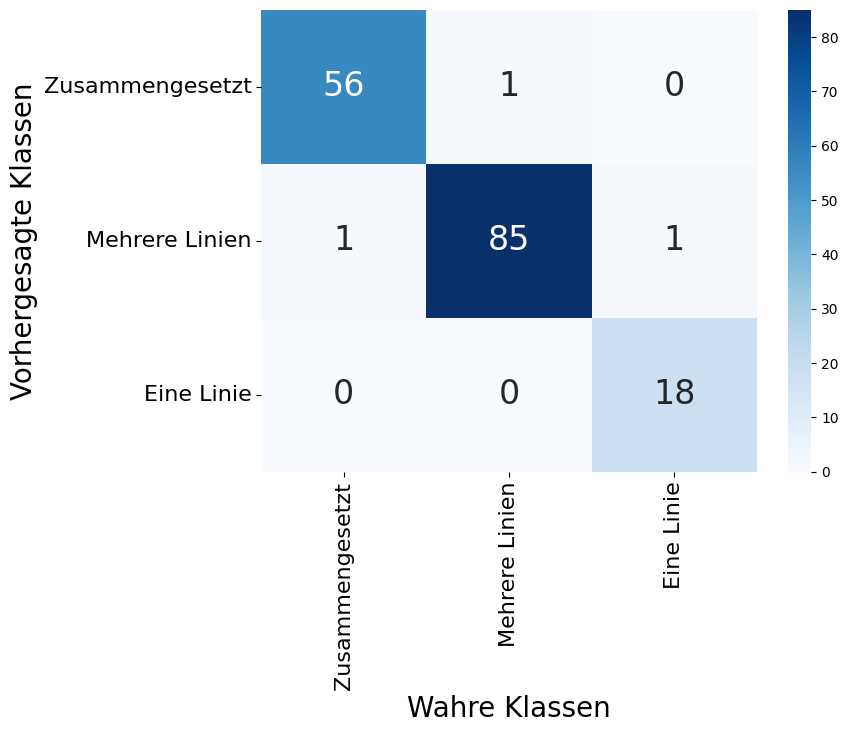
\includegraphics[width=.75\textwidth]{Experimente/img/classify/val_v2/matrix.png}
    \caption{\hbadness=10000 x}
    \label{fig:val_v2_matrix}
\end{figure}

\section{Segmentation}
\subsection{Instanzsegmentation durch Ultralytics YOLO}
\begin{table}[H]
    \centering
    \begin{tabular}{|l|c|c|c|}
        \hline
        \rowcolor[HTML]{EFEFEF}
              & Precision & Recall & F1-Score \\ \hline
        Box   & 95.6\%    & 78.8\% & 86.4\%   \\ \hline
        Maske & 93.3\%    & 76.4\% & 84.0\%   \\ \hline
    \end{tabular}
    \caption{x}
\end{table}

\subsection{Semantische Segmentation durch das U-Net}
\label{ch:eval_unet}

Mit den genannten Parametern aus \ref{ch:unet} wurden insgesamt fünf verschiedene Modelle trainiert: Eines wurde auf den in \ref{ch:lines} beschriebenen Binärmaskendatensatz der Wertelinien von synthetischen Liniendiagrammen vortrainiert. Die restlichen vier Modelle wurden auf den Werteliniendatensatz der historischen Liniendiagrammen so trainiert, um jeweils den Vergleich zwischen dem Fein- und nicht Feintrainieren und der selbst eingeführten Beschreibung des \emph{32x Batch-Paddings} darzustellen. Was dieses Batch-Padding beschreibt ist lediglich die 32-fache Duplikation aller einzelnen Trainingsdatenbilder. Da jeder einzelne Bilderbatch während des Trainingsprozesses zufällig neu augmentiert wird, und so durch das Batch-Padding die limitierten Trainingsdaten möglicherweise künslich vergrößern werden könnten, wurde dies untersucht.
\\
Alle im folgenden dargestellte Ergebnisse wurden auf denselben, den der historischen Diagrammswertelinien, Validationsdatensatz evaluiert. Um die Effizienz des erstellten Datensatzgenerators anschaulich zu machen wurde das auf den synthetischen Bildern vortrainiere Modell ebenfalls auf diesem Validationsdatensatz gemessen. Allerdings wurden hier keine herausragenden Evaluationswerte erwartet, da synthetische Datensätze in der Regel nicht die Qualität von realen Daten erreichen können.

\begin{table}[H]
    \centering
    \begin{minipage}{0.475\textwidth}
        \centering
        \begin{tabular}{|l|c|c|c|}
            \hline
            \rowcolor[HTML]{EFEFEF}
                  & Precision & Recall  & F1-Score \\ \hline
            Maske & 75.55\%   & 66.19\% & 70.56\%  \\ \hline
        \end{tabular}
        \caption{Training auf synthetischem Datensatz}
    \end{minipage}%
\end{table}

Die Tauglichkeit dieser künstlichen Herangehensweise zum lediglichen Vortrainieren spiegelt sich jedoch in den unteren Tabellen wider. Besonders der Precision Wert zwischen vor- und nicht vortrainierten Modellen zeigt Verbesserungen, hier in beiden Fällen von fast 1.5\%. Recall scheint davon nicht ganz betroffen zu sein, die Verbesserungen bei dem einen und Verschlechterungen bei dem anderen können allerdings der Zufälligkeitfaktoren des Trainings verschuldet sein. Die gleichen Auffälligkeiten können im Fall des Batch-Paddings gefunden werden.

\begin{table}[H]
    \centering
    \begin{minipage}{0.475\textwidth}
        \centering
        \begin{tabular}{|l|c|c|c|}
            \hline
            \rowcolor[HTML]{EFEFEF}
                  & Precision & Recall  & F1-Score \\ \hline
            Maske & 91.52\%   & 89.36\% & 90.43\%  \\ \hline
        \end{tabular}
        \caption{Training auf vortrainiertem Modell mit 32x Batch-Padding}
    \end{minipage}%
    \hfill
    \begin{minipage}{0.475\textwidth}
        \centering
        \begin{tabular}{|l|c|c|c|}
            \hline
            \rowcolor[HTML]{EFEFEF}
                  & Precision & Recall  & F1-Score \\ \hline
            Maske & 90.41\%   & 89.57\% & 89.99\%  \\ \hline
        \end{tabular}
        \caption{Training auf vortrainiertem Modell ohne 32x Batch-Padding}
    \end{minipage}

    \vspace{1.5em} % Adjust the spacing between the rows if needed

    \begin{minipage}{0.475\textwidth}
        \centering
        \begin{tabular}{|l|c|c|c|}
            \hline
            \rowcolor[HTML]{EFEFEF}
                  & Precision & Recall  & F1-Score \\ \hline
            Maske & 89.07\%   & 89.64\% & 89.35\%  \\ \hline
        \end{tabular}
        \caption{Training auf nicht vortrainiertem Modell mit 32x Batch-Padding}
    \end{minipage}%
    \hfill
    \begin{minipage}{0.475\textwidth}
        \centering
        \begin{tabular}{|l|c|c|c|}
            \hline
            \rowcolor[HTML]{EFEFEF}
                  & Precision & Recall  & F1-Score \\ \hline
            Maske & 88.05\%   & 88.88\% & 88.46\%  \\ \hline
        \end{tabular}
        \caption{Training auf nicht vortrainiertem Modell ohne 32x Batch-Padding}
    \end{minipage}
\end{table}

\section{Diagrammauswertung}

Da sich die Diagrammauswertung aus der Werteliniensegmentation und Achsenerkennung durch OCR zusammensetzt wurde nach obiger Evaluation des U-Nets ebenfalls die Effizienz des anderen Algorithmusteils beurteilt. Abgerundet wird das Kapitel der Experimente mit der Analyse des Diagrammauswertungsalgorithmus im Ganzen. Als Evaluationsdatensatz wurde für dieses gesamte Kapitel die durch \ref{ch:classify} implementierte und in \ref{ch:classify_eval} evaluierten Liniendiagrammsklassen der einer und mehreren Wertelinien verwendet. Wurden  Instanzen dieser falsch klassifiziert, so wurden diese bei den folgenden Auswertungen ignoriert.

\subsection{Achsenerkennung durch OCR}
\label{ch:eval_ocr}

Die Funktionsweise der Achsenerkennung durch optischer Schriftzeichenerkennung ist stark von der OCR selbst abhängig. Die Qualität der Erkennungen variiert stark durch die jeweilig verwendete OCR-Bibliothek, weswegen im Folgenden evaluierte Fehler in zwei, möglicherweise überlappende, Kategorien eingeteilt wurden. Diese bestehen aus den Fehlern des Algorithmus selbst, welche auch bei state-of-the-art Schriftzeichenerkennungsmethoden aufkommen würden. Da der Algorithmus das Auffinden der X-Achse im unteren Bildrand annimt, kommen eventuelle Fehler dieser Kategorie durch Diagramme mit anderen X-Achsen Positionen auf. Die andere Fehlergruppe sind der optischen Schriftzeichenerkennung selbst verschuldet, welche in Theorie durch eine bessere OCR-Bibliothek negiert werden kann.
\\
Es wurden 53 zufällige Diagramme manuell evaluiert, bei denen insgesamt 26 davon die korrekte Achsen- und Achsenbeschriftungserkennung erfüllten. Die Fehlerquellen der restlichen 27 Bilder werden in den unteren Tabellen dargestellt.

\begin{table}[H]
    \centering
    \begin{tabular}{|c|c|c|c|}
        \hline
        \rowcolor[HTML]{EFEFEF}
        Titel & Linke Y-Achse & Rechte Y-Achse & X-Achse \\ \hline
        3     & 0             & 1              & 7       \\ \hline
    \end{tabular}
    \caption{Von den 27 Fehlern wegen fehlerhaftem Achsenerkennungsalgorithmus}
    \label{tb:ocr1}
\end{table}

\begin{table}[H]
    \centering
    \begin{tabular}{|c|c|c|c|}
        \hline
        \rowcolor[HTML]{EFEFEF}
        Titel & Linke Y-Achse & Rechte Y-Achse & X-Achse \\ \hline
        6     & 6             & 4              & 10      \\ \hline
    \end{tabular}
    \caption{Von den 27 Fehlern wegen fehlerhafter optischer Schriftzeichenerkennung}
    \label{tb:ocr2}
\end{table}

\subsection{Numerische Tabellenformextraktion}

Letztendlich wurde der kombinierte und gesamte Tabellenformextraktionsalgorithmus evaluiert. Da der Algorithmus jedoch mit einigen Einschränkungen entworfen und seine einizgen Komponenten bereits oben in \ref{ch:eval_unet} und \ref{ch:eval_ocr} ausgewertet wurden, wurden einige Entscheidungen für die Algorithmusevaluation getroffen. Es soll die Effizienz des Algorithmus selbst bewertet werden, Fehler die aufgrund von ihm unausgelegter Problemen entstehen werden nicht in die Evaluation miteinbezogen. Folgende Annahmen wurden vorausgesetzt:
\\
Inkorrektheiten verursacht durch die primitive Wertelinientrennung bleiben unbeachtet, Fehler und Folgefehler der in \ref{ch:eval_ocr} beschriebener optischer Schriftzeichenerkennung werden ignoriert und die Bewertung wird unabhängig des korrekten Linientitels der Legende durchgeführt. Außerdem werden alle Werte anhand der Mitte des jeweiligen X-Achsen Labels abgelesen und nicht, wie korrekt, am eigentlichen respektiven Jahresende.
\\
Fehler werden durch der in \ref{ch:eval_ocr} genannten, fehlerhaften Achsenerkennungsalgorithmus gezählt, sowie bei falscher Y-Wert Auswertung, die möglicherweise durch falscher Interpolation der Y-Achse bei Diagrammen mit beispielweiser logarithmischen Skala auftreten kann. Desweiteren werden Fehler bei der falschen Werteliniensegmentation bestimmt, wie etwa beim Auftreten von Lücken oder irrtümlicher Erkennung in der Segmentierungsmaske.
\\
Insgesamt wurden 42 zufällig ausgewählte Liniendiagramme basierend auf den zuvor genannten Umständen manuell evaluiert.
\\
Die durchschnittliche Precision dabei lieg bei 91.64\% und die des Recalls bei 90.41\%.


\begin{figure}[H] % or any other figure positioning (H, h, t, b)
    \centering
    \begin{minipage}{0.475\textwidth} % First figure
        \centering
        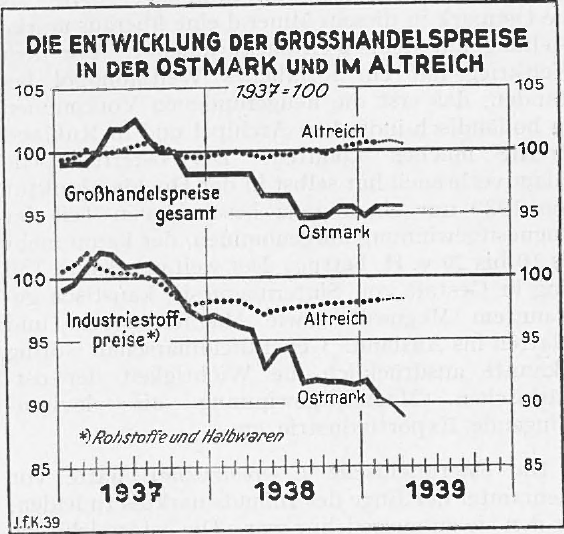
\includegraphics[width=\linewidth]{Experimente/img/f1.png}
        \caption{\hbadness=10000 Liniendiagramm mit komplexer Y-Achse}
        \label{fig:f1}
    \end{minipage}\hfill % Add space between figures
    \begin{minipage}{0.475\textwidth} % Second figure
        \centering
        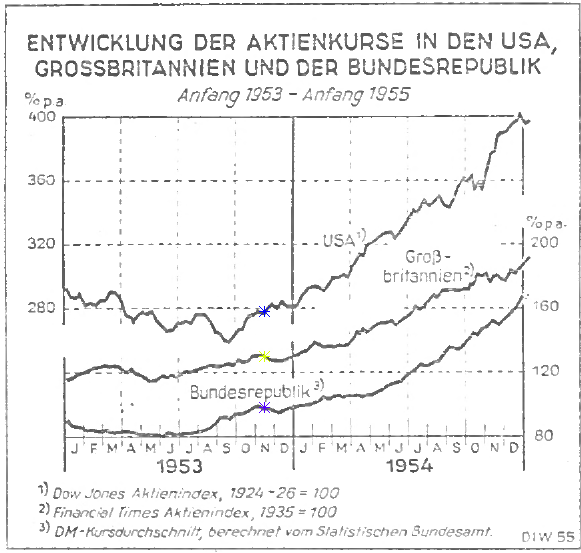
\includegraphics[width=\linewidth]{Experimente/img/f2.png}
        \caption{\hbadness=10000 Liniendiagramm mit unüblicher X-Achse}
        \label{fig:f2}
    \end{minipage}
\end{figure}

Fehlergründe lagen hier bei vereinzelt vorkommenden Lücken in der Werteliniensegmentation, aber der Großteil war dem Achsenerkennungsalgorithmus verschuldet. Abbildungen \ref{fig:f1} und \ref{fig:f2} zeigen Beispiele von zu Fehler führenden Diagrammen. Bei \ref{fig:f1} wird die Y-Achse nach Erreichen des Werts 100 auf 95 zurückgesetzt um zwei weitere Wertelinien einzubringen, welches Fehler in der der linearen Y-Wert Interpolation hervorruft. Bei \ref{fig:f2} dagegen schlägt die Erkennung der X-Achsen fehl, da diese sich unüblicherweise nicht mehr im unteren Rand des Bildes befindet.





% Im Kapitel "Experimente" Ihrer Bachelorarbeit sollten Sie die durchgeführten Versuche, deren Ergebnisse und Ihre Analyse darlegen. Hier ist eine Übersicht der wichtigsten Punkte, die in diesem Kapitel enthalten sein sollten:

% Versuchsaufbau:

% Beschreibung der verwendeten Datensätze (Trainings-, Validierungs- und Testdaten)
% Erklärung der Evaluierungsmetriken (z.B. mAP für YOLO, IoU für U-Net)
% Definition der Baseline oder Vergleichsmodelle


% Durchgeführte Experimente:

% Detaillierte Beschreibung jedes einzelnen Experiments
% Begründung für die Wahl der Experimente
% Variationen in Hyperparametern, Modellarchitekturen oder Trainingsmethoden


% Ergebnisse:

% Präsentation der quantitativen Ergebnisse (in Tabellen oder Grafiken)
% Qualitative Ergebnisse (z.B. Beispielbilder von Vorhersagen)
% Vergleich der Leistung von YOLO und U-Net für Ihre spezifische Aufgabe


% Analyse:

% Interpretation der Ergebnisse
% Diskussion von Stärken und Schwächen der Modelle
% Vergleich mit dem aktuellen Stand der Technik oder anderen relevanten Arbeiten


% Ablationstudie:

% Untersuchung des Einflusses verschiedener Komponenten oder Hyperparameter auf die Modellleistung


% Fehleranalyse:

% Identifikation von häufigen Fehlertypen
% Diskussion möglicher Gründe für diese Fehler


% Laufzeitanalyse und Ressourcenverbrauch:

% Vergleich der Inferenzzeiten von YOLO und U-Net
% Analyse des Speicher- und Rechenbedarfs


% Diskussion der Limitationen:

% Grenzen der durchgeführten Experimente
% Mögliche Verzerrungen in den Daten oder der Evaluation


% Zukünftige Arbeiten:

% Vorschläge für weitere Experimente oder Verbesserungen basierend auf Ihren Ergebnissen



% Dieses Kapitel sollte eine objektive Darstellung Ihrer experimentellen Arbeit sein, die es dem Leser ermöglicht, die Leistung und Eignung von YOLO und U-Net für Ihre spezifische Anwendung zu verstehen und zu bewerten.